\documentclass[tikz]{standalone}
\usepackage{lmodern,mathptmx,amsmath}
\usepackage{pbox}
\usepackage{marvosym}
\usepackage{bm}
\usepackage{wasysym}
\usepackage{makecell}
\usepackage{graphicx}
\usepackage{icomma}
\usepackage{afterpage}
\usepackage{pdflscape}
\usepackage{rotating}
\usepackage{pgfplots}
% \usepackage[T1]{fontenc}
% \usepackage[utf8]{inputenc}
\usepackage{pgfplots}
\usepackage{amsopn}
\usepackage{amsfonts}
\usepackage{amsthm, amsfonts, amssymb}
\usepackage{fontspec}
\defaultfontfeatures{Mapping=tex-text}
\setmainfont[Mapping=tex-text]{Latin Modern Roman}
\DeclareMathAlphabet{\mathcal}{OMS}{cmsy}{m}{n}
\DeclareMathOperator*{\unidist}{U}
\DeclareMathOperator*{\cov}{cov}
\DeclareMathOperator*{\argmax}{arg\,max}
\DeclareMathOperator*{\argmin}{arg\,min}
\DeclareMathOperator*{\sk}{sk}
\DeclareMathOperator*{\ku}{ku}
\DeclareMathOperator*{\qnc}{\#nc}
\DeclareMathOperator*{\qnom}{\#no}
\DeclareMathOperator*{\qnum}{\#nu}
\DeclareMathOperator*{\qatt}{\#at}
\DeclareMathOperator*{\qexe}{\#ex}
\DeclareMathOperator*{\qexeatt}{\#ea}
\DeclareMathOperator*{\lgqexe}{lgex}
\DeclareMathOperator*{\lgqexeatt}{lgea}
\DeclareMathOperator*{\nom}{isnom}
\DeclareMathOperator*{\pno}{\%no}
\DeclareMathOperator*{\en}{en}
\DeclareMathOperator*{\corr}{cr}
\DeclareMathOperator*{\cn}{cn}
\DeclareMathOperator*{\cnk}{cnk}
\DeclareMathOperator*{\si}{si}
\DeclareMathOperator*{\sik}{sik}
\DeclareMathOperator*{\du}{du}
\DeclareMathOperator*{\duk}{duk}
\DeclareMathOperator*{\dime}{dim}
\DeclareMathOperator*{\info}{Inf_\theta}
\DeclareMathOperator*{\stratID}{ID_\theta}
\DeclareMathOperator*{\stratIDTU}{ID_{TU}_\theta}
\DeclareMathOperator*{\JS}{JS}
\DeclareMathOperator*{\at}{\bm{a}}
\DeclareMathOperator*{\simi}{sim}
\DeclareMathOperator*{\limiar}{limite}
\DeclareMathOperator*{\limiaring}{max}
\begin{document}
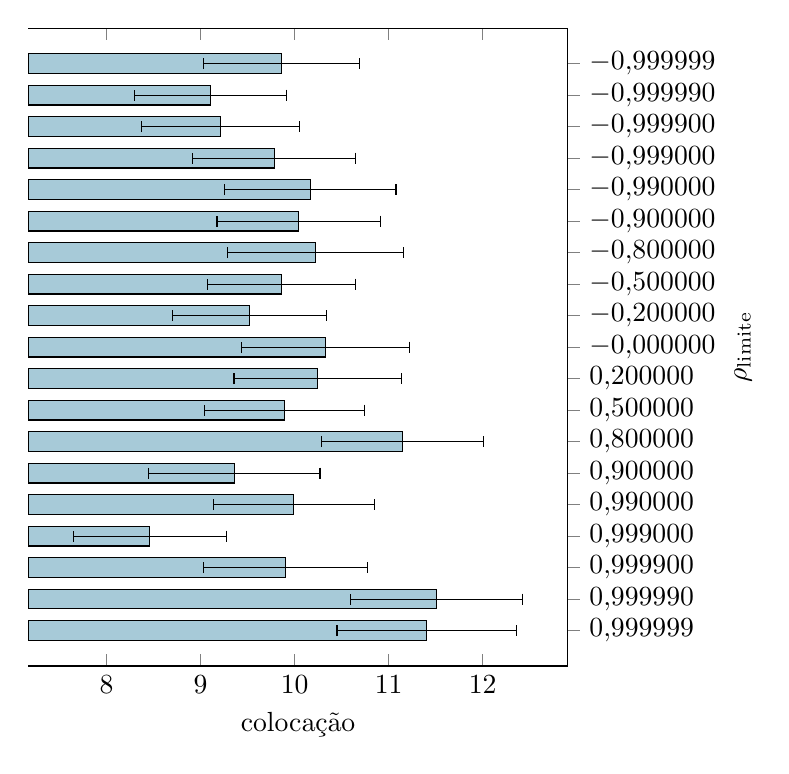
\begin{tikzpicture}
\begin{axis}[xbar,
  y=-0.4cm, bar width=0.25cm,
  enlarge y limits={abs=0.45cm}, ytick={1,2,3,4,5,6},
yticklabels={{$-0,999999$},{$-0,999990$},{$-0,999900$},{$-0,999000$},{$-0,990000$},{$-0,900000$},{$-0,800000$},{$-0,500000$},{$-0,200000$},{$-0,000000$},{$0,200000$},{$0,500000$},{$0,800000$},{$0,900000$},{$0,990000$},{$0,999000$},{$0,999900$},{$0,999990$},{$0,999999$}},
    xlabel={colocação},
    ylabel={$\rho_{\limiar}$},
     ytick=data,
%     nodes near coords,
%     nodes near coords align=horizontal,
    axis y line*=right] %, xmax=13,xmin=8]
\addplot [draw=black,fill=cyan!60!black!40, error bars/.cd,x dir=both,x explicit] table[x error=error] {
x y desv rho error
9.861702127659575	1	5.174588579209119	-0.999999	0.8280914243419962
9.106382978723405	2	5.06032020132345	-0.99999	0.8098050113543468
9.207446808510639	3	5.250401712469392	-0.9999	0.8402238295650072
9.78191489361702	4	5.431666663683183	-0.999	0.869231730258216
10.164893617021276	5	5.708128658698916	-0.99	0.9134740509228665
10.042553191489361	6	5.42825125530208	-0.9	0.8686851611256707
10.22340425531915	7	5.860207077920603	-0.8	0.937811219541635
9.856382978723405	8	4.92067305717634	-0.5	0.7874572245241622
9.52127659574468	9	5.1110858291345185	-0.2	0.8179290545315356
10.329787234042554	10	5.601724576754356	0	0.8964461642755498
10.24468085106383	11	5.557976289503505	0.2	0.8894451088394444
9.893617021276595	12	5.3066565727190635	0.5	0.84922631674582
11.148936170212766	13	5.394556090656281	0.8	0.8632929108128464
9.356382978723405	14	5.703527648455509	0.9	0.9127377494628465
9.98936170212766	15	5.348087148442394	0.99	0.8558564679040953
8.457446808510639	16	5.082470175863119	0.999	0.8133496804009624
9.898936170212766	17	5.456366404482745	0.9999	0.8731844393918016
11.51063829787234	18	5.731904074509423	0.99999	0.9172788399686954
11.404255319148936	19	5.961920649135168	0.999999	0.9540884819312284
% List(multiple-features, appendicitis, optdigits, micro-mass-pure-spectra, hayes-roth, cnae-9, breast-tissue-4class, qualitative-bankruptcy, texture, fertility-diagnosis, acute-inflammations-urinary, musk, digits2-davi, lsvt-voice-rehabilitation, micro-mass-mixed-spectra)
};
\end{axis}
\end{tikzpicture}
\end{document}